\documentclass[10pt,dvipdfmx]{standalone}
% \documentclass[10pt,dvipdfmx,b5paper,papersize]{jsarticle}
\usepackage{tikz}
\usetikzlibrary{intersections, calc}
\usetikzlibrary{arrows.meta}
\usepackage{physics}


\begin{document}

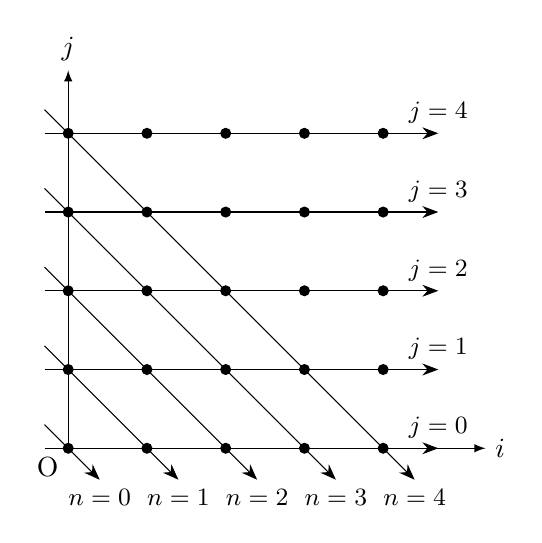
\begin{tikzpicture}[x=10mm,y=10mm,>=latex]
  % \small % 文字サイズ
  
  % 座標系
  \draw[->] (0,0) -- (5.3,0) node[right]{$i$}; % x軸
  % \draw[->] (0,0) -- (0,5.5) node[above]{$j$}; % y軸
  \draw[->] (0,0) -- (0,4.8) node[above]{$j$}; % y軸
  \node(O) at (0,0) [below left]{O}; % 原点

  %
  \foreach \x in {0,...,4} {
    \foreach \y in {0,...,4} {
      \fill (\x,\y) coordinate (P) circle[radius=2pt];
    }
  }
  % \foreach \n in {0,...,4} {
  %   \draw [domain=-0.3:\n+0.3, samples=50] plot(\x, -\x+\n) node[below]{{\small $n=\n$}};
  %   \draw [arrows= {-Stealth[scale=1.2]}] (0,\n) -- (4.8,\n) node[above]{{\small $j=\n$}};
  % }

  \foreach \n in {0,...,4} {
    \draw [arrows= {-Stealth[scale=1.2]},domain=-0.3:\n+0.4, samples=50] plot(\x, -\x+\n) node[below]{{\small $n=\n$}};
    \draw [arrows= {-Stealth[scale=1.2]}] (-0.3,\n) -- (4.7,\n) node[above]{{\small $j=\n$}};
  }

  

\end{tikzpicture}




\end{document}